\documentclass[border=10pt]{standalone}

\usepackage{tikz}
\usepackage{tikzsymbols}
\usetikzlibrary{calc,patterns,shapes.geometric}

\def\centerarc[#1](#2)(#3:#4:#5){\draw[#1] ($(#2)+({#5*cos(#3)},{#5*sin(#3)})$) arc (#3:#4:#5);}

\begin{document}
	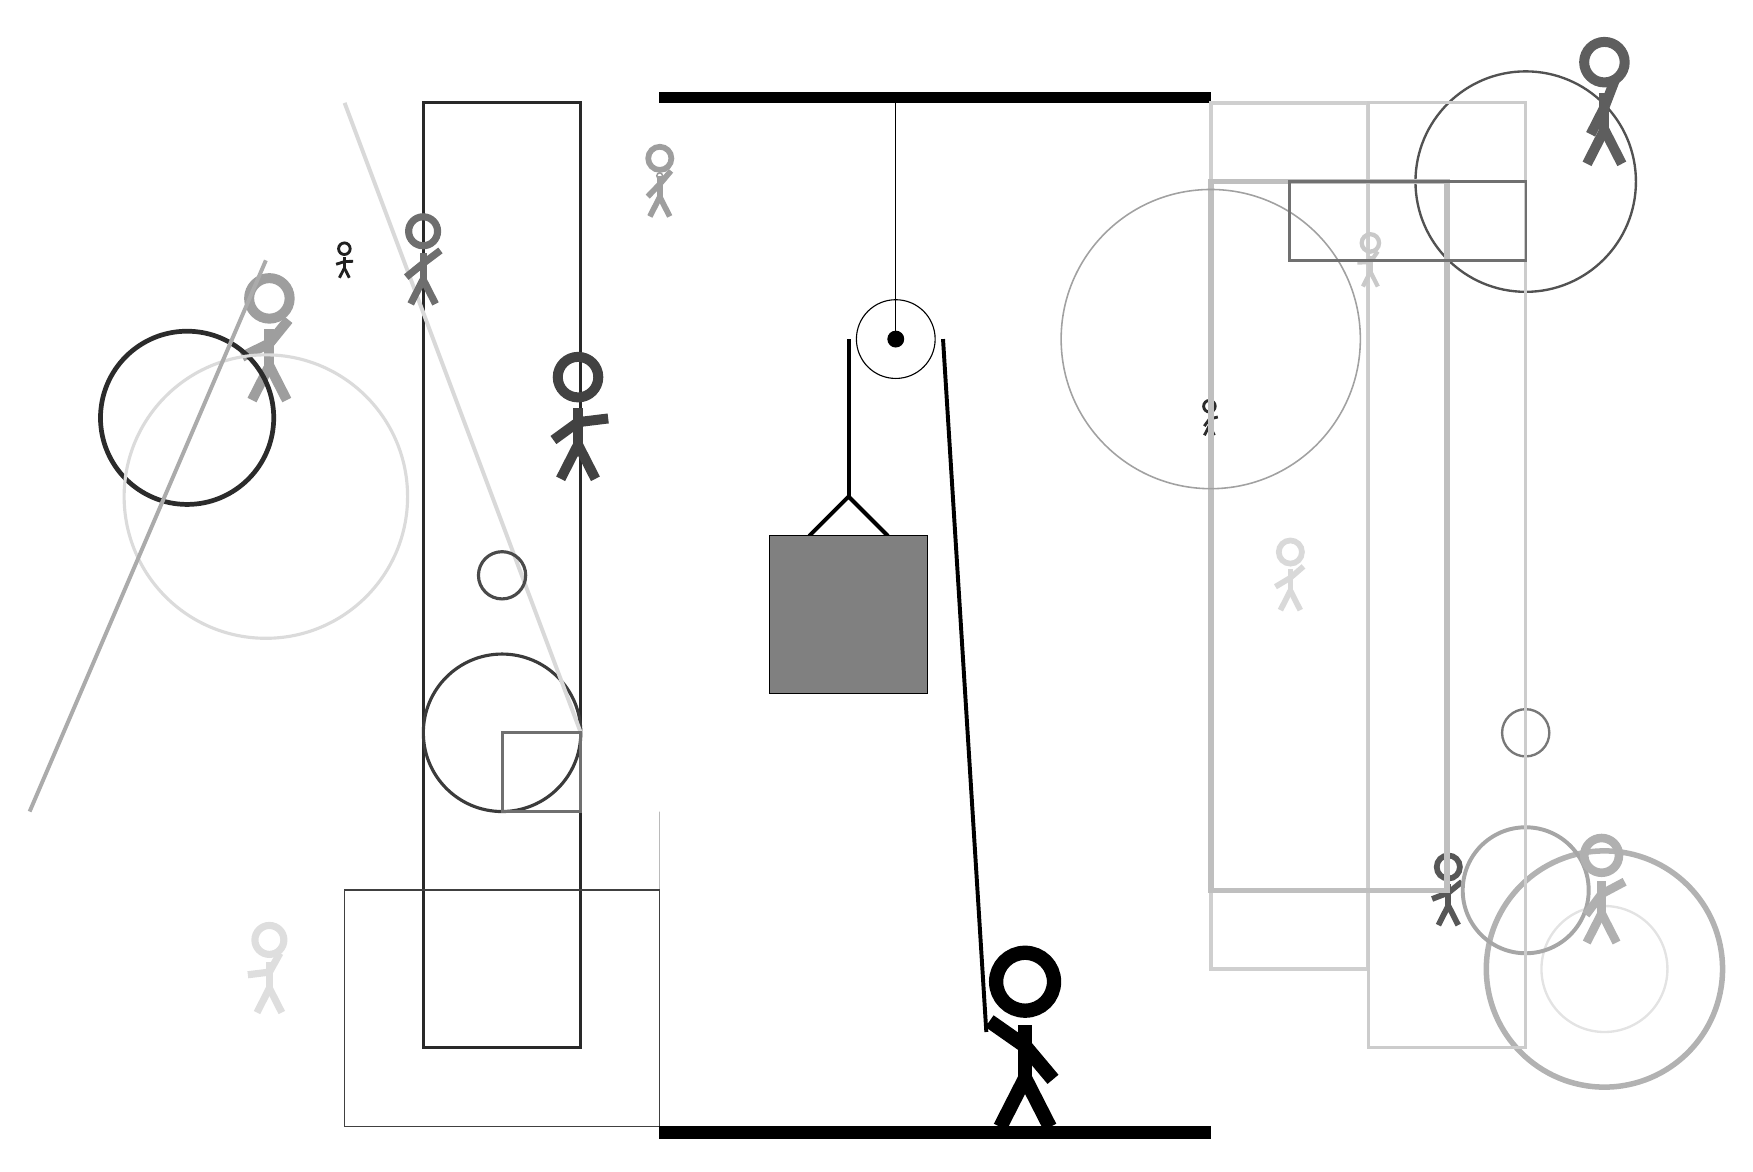
\begin{tikzpicture}
		%%%%% START %%%%%
		
		\draw[fill=black] (-2, 10) rectangle (5, 10.125);
		
		\draw (1, 7) circle (0.5);
		\draw[fill=black] (1, 7) circle (0.1);
		\draw (1, 10) -- (1, 7);
		
		\draw[line width=0.5mm] (-0.1, 4.5) -- (0.4, 5.0) -- (0.9, 4.5);
		\draw[fill=black!50] (-0.6, 4.5) rectangle (1.4, 2.5);
		
		\draw [line width=0.3mm, color=black!53](9, 2) circle (0.3);
		
		\node[line width=0.7mm, color=black!38] at (-7, 7) {\Strichmaxerl[7][26][51]};
		\node[line width=0.3mm, color=black!40] at (-2, 9) {\Strichmaxerl[1][45][80]};
		\node[line width=0.7mm, color=black!38] at (-2, 9) {\Strichmaxerl[4][46][50]};
		
		\draw [line width=0.6mm, color=black!83](-8, 6) circle (1.1);
		\node[line width=0.4mm, color=black!66] at (8, 0) {\Strichmaxerl[4][21][39]};
		
		\draw [line width=0.4mm, color=black!14](-7, 5) circle (1.8);
		\draw[line width=0.4mm, color=black!84] (-3, -2) rectangle (-5, 10);
		\draw [line width=0.7mm, color=black!30](10, -1) circle (1.5);
		
		\draw [line width=0.3mm, color=black!11](10, -1) circle (0.8);
		\draw [line width=0.3mm, color=black!68](9, 9) circle (1.4);
		
		\draw[line width=0.5mm, color=black!19] (5, -1) rectangle (7, 10);
		\node[line width=0.2mm, color=black!74] at (-3, 6) {\Strichmaxerl[7][36][7]};
		\draw[line width=0.5mm, color=black!33](-7, 8) -- (-10, 1);
		\node[line width=0.6mm, color=black!15] at (6, 4) {\Strichmaxerl[4][31][41]};
		\draw [line width=0.5mm, color=black!35](9, 0) circle (0.8);
		
		\node[line width=0.5mm, color=black!13] at (-7, -1) {\Strichmaxerl[5][7][61]};
		
		\draw [line width=0.4mm, color=black!77](-4, 2) circle (1.0);
		\draw[line width=0.2mm, color=black!27] (-2, 1) rectangle (-2, -2);
		
		\draw[line width=0.2mm, color=black!75] (-2, -3) rectangle (-6, 0);
		\node[line width=0.7mm, color=black!83] at (5, 6) {\Strichmaxerl[2][54][14]};
		\node[line width=0.4mm, color=black!87] at (-6, 8) {\Strichmaxerl[2][18][2]};
		
		\draw[line width=0.5mm, color=black!15](-3, 2) -- (-6, 10);
		\draw[line width=0.4mm, color=black!20] (7, -2) rectangle (9, 10);
		\draw [line width=0.4mm, color=black!71](-4, 4) circle (0.3);
		
		\node[line width=0.3mm, color=black!31] at (10, 0) {\Strichmaxerl[6][53][28]};
		
		\draw[line width=0.7mm, color=black!25] (5, 9) rectangle (8, 0);
		\node[line width=0.3mm, color=black!57] at (-5, 8) {\Strichmaxerl[5][39][37]};
		
		\draw[line width=0.4mm, color=black!56] (-3, 1) rectangle (-4, 2);
		\draw [line width=0.2mm, color=black!37](5, 7) circle (1.9);
		\node[line width=0.4mm, color=black!21] at (7, 8) {\Strichmaxerl[3][1][56]};
		
		\draw[line width=0.3mm, color=black!56] (6, 9) rectangle (9, 8);
		\node[line width=0.4mm, color=black!63] at (10, 10) {\Strichmaxerl[7][63][69]};
		
		
		\draw[line width=0.5mm] (0.4, 7) -- (0.4, 5.0);
		\centerarc[line width=0.5mm](1, 7)(0:180:0.6);
		\draw[line width=0.5mm](1.6, 7) -- (2.15, -1.8);
		
		\node at (2.6, -1.9) {\Strichmaxerl[10][-35][-50]};
		
		\draw[fill=black] (-2, -3) rectangle (5, -3.15);
		
		%%%%% END %%%%%
	\end{tikzpicture}
\end{document}